\documentclass{article}[12pt]
\renewcommand{\baselinestretch}{1.5}
\setlength{\parskip}{1em}

\usepackage[parfill]{parskip}
\usepackage[affil-it]{authblk}
\usepackage[space]{grffile}

\usepackage[a4paper]{geometry}
\geometry{verbose}
\usepackage{float}
\usepackage{graphicx}
\usepackage{setspace}
\usepackage{caption}

\usepackage[utf8]{inputenc}
\usepackage[english]{babel}

\usepackage{latexsym,textcomp,longtable,tabulary}
\usepackage{booktabs,array,multirow,braket}
\usepackage{amsfonts,amsmath,amssymb,mathbbol,calc,cancel}
\usepackage{subfigure,color,blindtext,enumitem,siunitx}
\usepackage[colorinlistoftodos]{todonotes}

\usepackage{mathtools}
\usepackage{url,hyperref,etoolbox}
\numberwithin{equation}{section}
\hypersetup{colorlinks=false,pdfborder={0 0 0}}

%+figure layout options
\restylefloat{figure}
\setlist{leftmargin=*,before=\setlength{\rightmargin}{\leftmargin}}
%-figure layout options

\providecommand\citet{\cite}
\providecommand\citep{\cite}
\providecommand\citealt{\cite}

\makeatletter
\makeatother

\begin{document}

\title{
	Inference and Synthesis of\\
	co-dimension one Bifurcations
}

\author{Gregory Szep$^{1,2}$, Neil Dalchau$^2$ and Attila Csikasz-Nagy$^1$}
\affil{$^1$King's College London, $^2$Microsoft Research Cambridge}
\date{\today}
\maketitle
\vspace{-25pt}
\section{Introduction and Motivation}

\begin{itemize}
\item qualitative equivalence more important
\item fitting to time courses not appropriate
\item gradient information makes optimisation tractable
\item similar works
\end{itemize}

\clearpage
\section{Problem Statement}
Suppose we parametrise a set of differential equations for states $u\in\mathbb{R}^N$ with a function $F_{\theta}$ in an unknown parameter space $\theta\in\mathbb{R}^M$. We would like these differential equations to obey 
a set of target bifurcations $\mathcal{D}:=\{p_1\dots p_K\}$ along a known bifurcation parameter $p\in\mathbb{R}$. The following sections outline how a gradient descent algorithm could encourage predicted bifurcations $\mathcal{P}(\theta)$ coming from parameterised differential equations to match specified targets $\mathcal{D}$. This would allow us to design differential equations using high-level qualitative constraints and sample qualitatively equivalent models in regions of optimal $\theta$. Let the differential equations be defined as
\begin{align}
	\partial_t u=F_{\theta}(z)
	\qquad\mathrm{where}\quad z:=(u,p)\quad
	F_{\theta} : \mathbb{R}^{N+1}\rightarrow\mathbb{R}^N
\end{align}

\section{Methodology}
First we view the steady states of this problem in terms of implicit space curves \cite{Goldman2005CurvatureSurfaces} in an augmented state space $z\in \mathbb{R}^{N+1}$ which combines the state $u$ and bifurcation parameter $p$. We then realise that it is possible to analytically evaluate the curvature of the determinant $\Delta_\theta(z)$, which when maximised encourages bifurcations in the region of $z$. In order to know which regions of $z$ need evaluation, a parameter continuation method \cite{Veltz2019PseudoArcLengthContinuation.jl,Farrell2016TheDiagrams} is used together with some pre-conditioning methods to ensure hyper-parameters remain constant. Finally a piecewise-differentiable semi-supervised objective function $L(\theta)$ is proposed that would allow gradient descent algorithms to efficiently encourage bifurcations and match their locations to targets $\mathcal{D}$.

For clarity we guide the reader through the methods with the following co-dimension one normal forms: the saddle-node $F_{\theta}(z) = p + \theta_{1}u+\theta_{2}u^3$ and pitchfork $F_{\theta}(z) = \theta_{1} + p u+\theta_{2}u^3$ with corresponding targets $\mathcal{D}$ as shown in Figure \ref{fig:saddle-node} and Figure \ref{fig:pitchfork} respectively. These figures show that the curvature of the determinant $\Delta_\theta(z)$ increases in the vicinity of bifurcations and crosses zero at the bifurcation. This gives us our first hint of what should be optimised to encourage bifurcations. Success on these normal forms demonstrates the proof of concept, and success in practice is demonstrated on more complicated genetic feedback systems taken from examples in synthetic biology.

\begin{figure}[H]
\centering{}
\captionsetup{justification=centering}
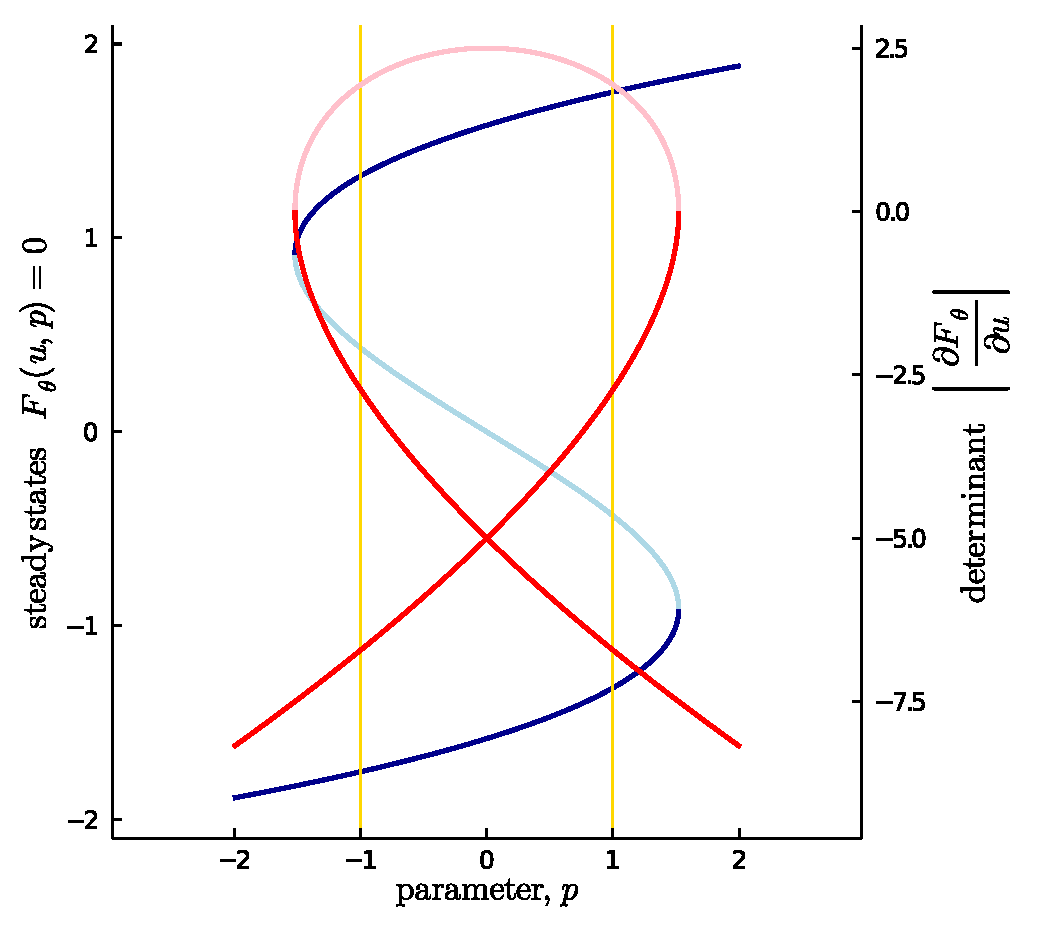
\includegraphics[width=11cm]{docs/figures/saddle-node}
\caption{Saddle-node normal form $F_{\theta}(z) = p + \theta_{1}u+\theta_{2}u^3$ with set $\theta=(2,-1)$ and targets $\mathcal{D}=\{-1/2,1/2\}$. Lighter shades indicate the determinant crossing zero for unstable solutions}
\label{fig:saddle-node}
\end{figure}

\begin{figure}[H]
\centering{}
\captionsetup{justification=centering}
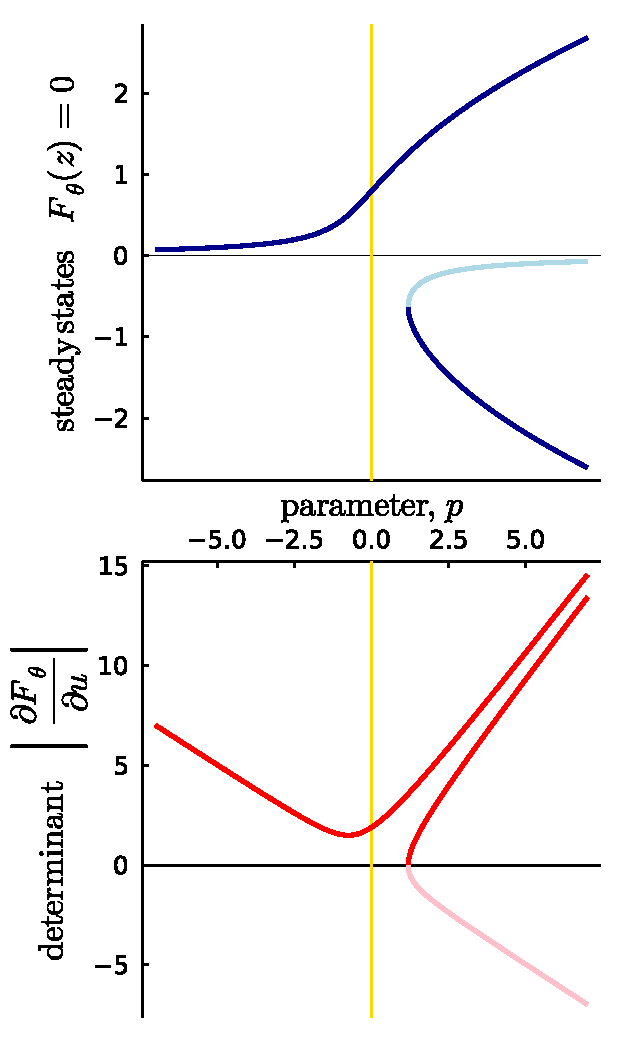
\includegraphics[width=11cm]{docs/figures/pitchfork}
\caption{Pitchfork normal form $F_{\theta}(z) = \theta_{1} + p u+\theta_{2}u^3$ with set $\theta=(-1/10,-1)$ and target $\mathcal{D}=\{0\}$. Lighter shades indicate the determinant crossing zero for unstable solutions}
\label{fig:pitchfork}
\end{figure}

\subsection{Co-dimension one bifurcations as implicit space curves}
Using 
The steady states define $N$ surfaces in $\mathbb{R}^{N+1}$ which may intersect to form an implicit space curve. This curve given by the following $N$ implicit equations
\begin{align}
    F_{\theta}(z) = 0
\end{align}
Let us first focus on one of the surfaces defined by $f_{\theta}(z)=0$ where $f_{\theta} : \mathbb{R}^{N+1}\rightarrow\mathbb{R}$. Since $f_{\theta}(z)=c$ defines an equipotential for any constant $c$ and the gradient vector $\partial_z f_{\theta}$ points in the direction of steepest ascent for $f_{\theta}$, then the gradient $\partial_z f_{\theta}$ must be perpendicular to all equipotentials $f_{\theta}(z)=c$ and therefore also perpendicular to surface defined by $f_{\theta}(z)=0$. Each surface therefore has a normal given by
$\partial_z f_{\theta}$ for values of $z$ that solve $f_{\theta}(z)=0$.
These normal vectors must all be perpendicular to the implicit space curve defined by the intersection of these surfaces \cite{Goldman2005CurvatureSurfaces}. This geometric constraint is illustrated by example in Figure \ref{fig:implicit-surfaces}.

\begin{figure}[H]
\centering{}
\captionsetup{justification=centering}
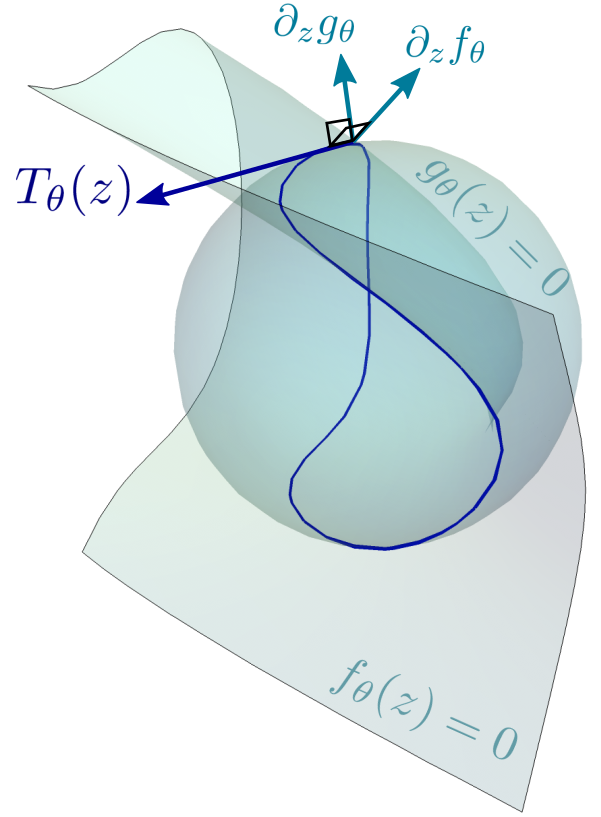
\includegraphics[width=8cm]{docs/figures/implicit-surfaces}
\caption{Implicit surfaces $f_{\theta}(z)=0$ and $g_{\theta}(z)=0$ in $\mathbb{R}^3$ intersecting to form\\ a space curve $T_{\theta}(z)$ that is perpendicular to their gradients $\partial_{z}f_{\theta}$ and $\partial_{z}g_{\theta}$}
\label{fig:implicit-surfaces}
\end{figure}

The tangent vector $T_{\theta}(z)$ to the implicit space curve can be constructed perpendicular to all gradient vectors using the properties of the determinant
\begin{align}
    T_{\theta}(z):=
    \left|\begin{matrix}
        \hat{z} \\
        \,\partial_{z}F_{\theta}\,
    \end{matrix}\right|
    \qquad\mathrm{where}\quad
    \hat{z}:=(\hat{u},\hat{p})\quad
	T_{\theta} : \mathbb{R}^{N+1}\rightarrow\mathbb{R}^{N+1}
\end{align}
where $\hat{z}$ is a collection of unit basis vectors in the $\mathbb{R}^{N+1}$ space and $\partial_{z}F_{\theta}$ is an $N\times(N+1)$ augmented Jacobian matrix of partial derivatives including $\partial_p F_{\theta}$ in the last column. The dot product of this tangent vector any individual gradient vector $\partial_z f_{\theta}$ distributes the components of the gradient across the columns
\begin{align}
    T_{\theta}(z)\cdot\partial_z f_{\theta}&=
    \left|\begin{matrix}
        \partial_z f_{\theta} \\
        \,\partial_{z}F_{\theta}\,
    \end{matrix}\right|\\&=0 \quad\forall f_{\theta}\in F_\theta
\end{align}

\begin{figure}[H]
\centering{}
\captionsetup{justification=centering}
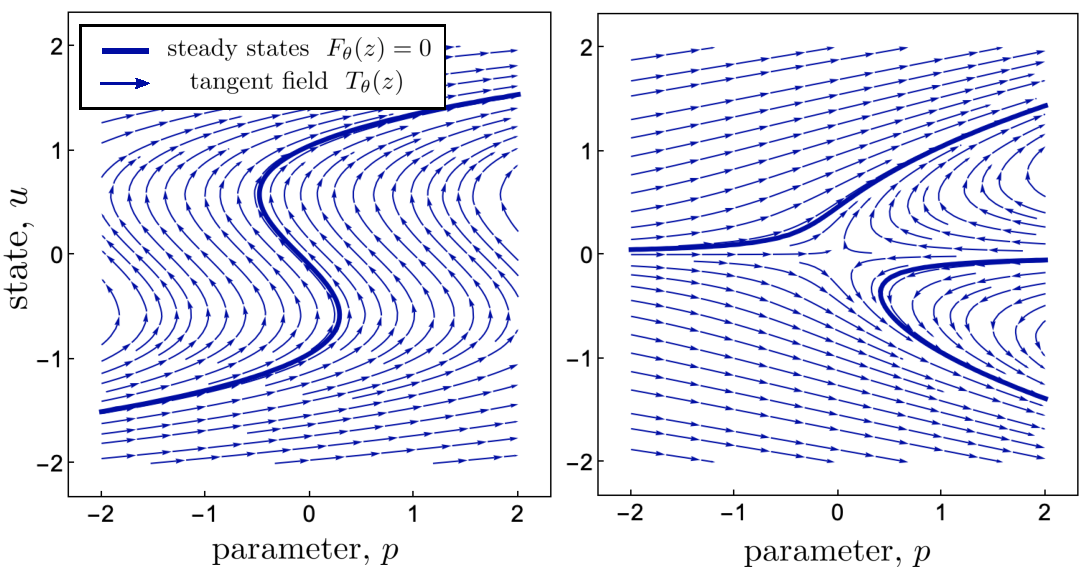
\includegraphics[width=14cm]{docs/figures/tangent-field}
\caption{Left/Right : Calculated tangent fields $T_{\theta}(z)$ for the saddle-node/pitchfork normal forms for some set value of $\theta$, revealing that $F_{\theta}(z)=0$ picks out one of the traces in the field}
\label{fig:tangent-field}
\end{figure}
The determinant of any matrix with two identical rows or columns is zero, satisfying our perpendicularity condition. Note that the vector field $T_{\theta}(z)$ is actually defined for all values of $z$, where adjacent field lines trace out other solutions where $F_{\theta}(z)\neq0$ which may be useful for understanding transient behaviour. Figure \ref{fig:tangent-field} shows how the solution $F_{\theta}(z)=0$ picks out one of many traces in tangent field $T_{\theta}(z)$ for the saddle and pitchfork. Since the tangent field $T_{\theta}(z)$ can always be analytically evaluated can proceed with calculations on the whole space $z$ and pick out a single trace by solving $F_{\theta}(z)=0$ later. The tangent fields for the saddle node and pitchfork are $T_{\theta}(z)=(\,3\theta_2 u^2-\theta_1\,)\,\hat{p}+\hat{u}$ and $T_{\theta}(z)=(\,3\theta_2 u^2-p\,)\,\hat{p}+u\hat{u}$ respectively.

\subsection{Evaluating Curvature of the Determinant}
Bifurcations are defined as values of $p$ where eigenvalues $\lambda$ of the Jacobian $\partial_u F(z)$ cross either the real or imaginary axis in the complex plane. Restricting our case for $\lambda\in\mathbb{R}$ for now, the determinant of the Jacobian
\begin{align}
    \Delta_\theta(z) := \big|\,\partial_u F_\theta\,\big|
\end{align}
crossing zero can be used as a readout of whether a bifurcation has occurred. Consequently the curvature of the determinant along the implicit space curve $F_{\theta}(z)=0$ increases in the vicinity of bifurcations as can be seen in Figure \ref{fig:saddle-node} and Figure \ref{fig:pitchfork}. The total determinant curvature along the implicit space curve can be calculated as
\begin{align}
    \kappa(\theta) := \int_{F_\theta(z)=0}\!|\partial_{T_\theta}^2\Delta_\theta|\,\mathrm{d}z
\end{align}
where $F_{\theta}(z)=0$ picks out an implicit space curve given by $\theta$. Here we note that the integrand as well as the limits are functions of $\theta$. The second directional derivative with respect to tangent field $T_\theta(z)$
\begin{align}
    \partial_{T_\theta}^2\Delta_\theta
    &:=
    \bigg(
        \partial_z\left(\partial_z\Delta_\theta\cdot \hat{T}_\theta\right)
    \bigg)\cdot \hat{T}_\theta\quad
    \mathrm{where}\quad\hat{T}_\theta:=\frac{T_\theta}{|T_\theta|}\\
    &=
        \hat{T}_\theta \cdot \partial_z^2\Delta_\theta \cdot \hat{T}_\theta+
        \partial_z\Delta_\theta\cdot \partial_z \hat{T}_\theta \cdot \hat{T}_\theta
\end{align}
The first term in the expression above is the usual result involving the Hessian matrix $\partial_z^2\Delta_\theta$ when taking second order directional derivatives. The second term appears because $\hat{T}_\theta(z)$ is a function of $z$ giving rise to a non-zero Jacobian matrix $\partial_z \hat{T}_\theta$. All these quantities are obtained by taking derivatives and determinants of $F_{\theta}(z)$ and in principle can always be done symbolically, giving us a closed analytical expression for the determinant curvature $\partial_{T_\theta}^2\Delta_\theta$. For the saddle-node and pitchfork the expression evaluates respectively to
\begin{align}
    \partial_{T_\theta}^2\Delta_\theta = 
    -\frac{6 \theta_2 \left(\theta _1^2-9 \theta _2^2 u^4+2\right)}
    {\left(\left(\theta _1+3 \theta _2 u^2\right){}^2+2\right){}^2}
    \qquad
    \partial_{T_\theta}^2\Delta_\theta =
    -\frac{2 u^2 \left(p+3 \theta _2 u^2\right) \left(9 \theta _2 \left(p+\theta _2 u^2\right)+2\right)}{\left(p^2+6 \theta _2 p u^2+9 \theta _2^2 u^4+2 u^2\right){}^2}
\end{align}
\subsection{Semi-supervised Objective Function}


\subsection{Hyper-parameter Preconditioning}


\section{Method}

\subsection{Pseudo-arclength Continuation}
\label{sec:continuation}

\begin{itemize}
    \item predictor-corrector algorithm
    \end{itemize}

\subsection{Optimization}

\subsubsection{Objective Function}
\label{sec:objective-function}

The objective function has two regimes: curvature-driven and target-driven. In
the curvature-driven regime the objective should seek to maximise the curvature
of $\mathcal{U}(\theta)$ anywhere within the target region containing points $\mathcal{D}$.
One curvature measure would be Kurtosis along $p$ - the fourth order standardised moment
\begin{align}
    \mathrm{Kurt}\left[\,\mathcal{U}(\theta)\,\right]:=
    \frac{1}{|\,\mathcal{U}(\theta)|}\sum_{(u,p)\in\mathcal{U}(\theta)}
    \left(\frac{p-\mu}{\sigma}\right)^4\qquad\qquad\quad\\
    \mathrm{where}\qquad
    \mu:=\!\!\!\!\!\!\sum_{(u,p)\in\mathcal{U}(\theta)}\!\!\!p/|\,\mathcal{U}(\theta)|
    \qquad
    \sigma^2:=\!\!\!\!\!\!\sum_{(u,p)\in\mathcal{U}(\theta)}\!\!\!(p-\mu)^2/|\,\mathcal{U}(\theta)|
\end{align}
The target-driven regime is only activated if there are a finite number of fold points $\mathcal{P}(\theta)$; in this case the objective function take a more familiar norm $|\,\mathcal{P}(\theta)-\mathcal{D}\,|^2$  which evaluates the distance between prediction
and target. The complete objective function is
\begin{align}
	\mathcal{J}(\theta):= \begin{cases}
	|\,\mathcal{P}(\theta)-\mathcal{D}\,|^2 & |\mathcal{P}(\theta)|>0 \\
	\mathbb{e}^{-\mathrm{Kurt}\left[\,\mathcal{U}(\theta)\,\right]} & \mathrm{otherwise}
	\end{cases}
\end{align}
In order to perform gradient descent on this objective we apply
\begin{align}
    \partial_\theta\mathcal{J}=\begin{cases}
	2(\mathcal{P}(\theta)-\mathcal{D})\,\partial_\theta\mathcal{P} & |\mathcal{P}(\theta)|>0 \\
	-\mathbb{e}^{-\mathrm{Kurt}\left[\,\mathcal{U}(\theta)\,\right]}\, \partial_\theta\mathcal{U}\,\mathrm{Kurt}'\left[\,\mathcal{U}(\theta)\,\right] & \mathrm{otherwise}
	\end{cases}
\end{align}
This objective function is differentiable --- except for at the boundary between
the two regimes --- if we can compute $\partial_\theta\mathcal{U}$ and $\partial_\theta\mathcal{P}$. This requires the algorithm in section \ref{sec:continuation} to be differentiable. This is where
\texttt{Zygote.jl}, a differentiable programming system that is able to take gradients of general program structures \cite{}, is applied.


\todo[inline]{Try adding a penalty for "conjugate stability"}
\todo[inline]{Comment that while reproducing the qualitative behaviour only can be desirable, sometimes it is also helpful to add quantitative desires over the values of the output. E.g. we don't care too much about [CFP], but actually, if it were below $C_\text{threshold}$, then we'd have a problem. This can be cast in terms of a multi-objective optimization problem, where each term separately gets a weighting factor. Personally, I wouldn't demonstrate that in this paper, but important to comment somewhere.}
\todo[inline]{Try applying the KDE function to the target output, as well as the model output.}

\subsubsection{Optimization details}

\begin{itemize}
    \item ADAM
\end{itemize}
\todo[inline]{Try removing momentum from the optimizer}

\section{Normal Forms}
\label{sec:normal-forms}

\begin{itemize}
    \item saddle-node, pitchfork, transcritical
    \item benchmarks against other algos
\end{itemize}


\section{Chemical Reaction Networks}
\label{sec:networks}

\begin{itemize}
    \item toggle switch
    \item cell cycle (Attila)
    \item application to structure $\rightarrow$ function (Luca)
\end{itemize}

\section{Conclusions and Extensions}
\label{sec:conclusions}

\begin{itemize}
    \item hyperparam optimization
    \item hopf bifurcations
    \item pattern formation in pdes (Neil)
\end{itemize}

\bibliography{refs}
\bibliographystyle{ieeetr}
\end{document}
